%% Patent Application: Pulse Protocol Methods for Resonant Protein Folding Modulation
%% Inventor: Jonathan Washburn
%% Contact: washburn.jonathan@gmail.com
%% Filing Date: January 2026

\documentclass[12pt,letterpaper]{article}

\usepackage[margin=1in]{geometry}
\usepackage{amsmath,amssymb,amsfonts}
\usepackage{graphicx}
\usepackage{tikz}
\usetikzlibrary{shapes,arrows,positioning,calc,patterns,decorations.pathmorphing}
\usepackage{booktabs}
\usepackage{array}
\usepackage{enumitem}
\usepackage{fancyhdr}
\usepackage{xcolor}
\usepackage{hyperref}
\usepackage{setspace}

% Patent-style formatting
\setlength{\parindent}{0.5in}
\setlength{\parskip}{0.5em}
\onehalfspacing

% Header
\pagestyle{fancy}
\fancyhf{}
\rhead{Patent Application}
\lhead{Washburn}
\rfoot{Page \thepage}

\hypersetup{
    colorlinks=true,
    linkcolor=blue,
    urlcolor=blue,
    citecolor=blue
}

% Custom colors
\definecolor{pulse}{RGB}{200,50,50}
\definecolor{folding}{RGB}{50,150,50}
\definecolor{temp}{RGB}{50,50,200}
\definecolor{detect}{RGB}{200,150,50}

\begin{document}

%% ============================================================================
%%                              TITLE PAGE
%% ============================================================================

\begin{center}
\vspace*{0.8in}

{\LARGE \textbf{PATENT APPLICATION}}

\vspace{0.4in}

{\Large \textbf{PULSE PROTOCOL METHODS FOR}}

{\Large \textbf{RESONANT PROTEIN FOLDING MODULATION}}

{\Large \textbf{AND INTERMEDIATE TRAPPING}}

\vspace{0.8in}

\textbf{PROVISIONAL PATENT APPLICATION}

\vspace{0.5in}

\begin{tabular}{ll}
\textbf{Inventor:} & Jonathan Washburn \\
\textbf{Email:} & washburn.jonathan@gmail.com \\
\textbf{Filing Date:} & January 17, 2026 \\
\textbf{Application Type:} & Utility Patent (Provisional) \\
\textbf{Related Applications:} & Patents 001--004 \\
\end{tabular}

\vspace{0.8in}

\textit{Methods for applying pulsed microwave irradiation at the jamming frequency to modulate protein folding, including synchronized pulse timing relative to folding initiation, duty cycle optimization, pulse trains for kinetic studies, frequency-chirped pulses, phase-locked detection schemes, intermediate trapping protocols, and isothermal pulsing control rules.}

\vfill

\textbf{CONFIDENTIAL --- PATENT PENDING}

\end{center}

\newpage

%% ============================================================================
%%                         TABLE OF CONTENTS
%% ============================================================================

\tableofcontents
\newpage

%% ============================================================================
%%                              ABSTRACT
%% ============================================================================

\section*{ABSTRACT OF THE DISCLOSURE}
\addcontentsline{toc}{section}{ABSTRACT OF THE DISCLOSURE}

Methods for applying pulsed electromagnetic radiation at a resonant jamming frequency (approximately 14.65 GHz for H$_2$O, 10.4 GHz for D$_2$O) to modulate protein folding dynamics. The methods comprise: (a) synchronized pulse timing relative to folding initiation events including temperature jump, rapid mixing, and pH jump; (b) duty cycle optimization to balance folding modulation against thermal load; (c) pulse train protocols for kinetic characterization of folding pathways; (d) frequency-chirped pulses for broadband resonance excitation; (e) phase-locked detection schemes for enhanced signal-to-noise ratio; (f) intermediate trapping protocols using precisely timed pulses to arrest folding at specific stages; and (g) isothermal pulsing control rules that maintain constant sample temperature despite pulsed irradiation. The methods enable precise temporal control of protein folding modulation, allow characterization of folding intermediates not accessible by continuous-wave irradiation, and provide enhanced discrimination between resonant and thermal effects. Pulse timing parameters are derived from the molecular gate timescale ($\tau_{19} \approx 68$ ps) and the Recognition Science framework. Applications include structural biology research, drug discovery, biopharmaceutical manufacturing quality control, and therapeutic intervention in protein misfolding diseases.

\vspace{1em}
\noindent\textbf{Keywords:} pulsed irradiation, protein folding, intermediate trapping, duty cycle, pulse train, chirp, phase-locked detection, isothermal pulsing, folding kinetics

\newpage

%% ============================================================================
%%                      BACKGROUND OF THE INVENTION
%% ============================================================================

\section{BACKGROUND OF THE INVENTION}

\subsection{Field of the Invention}

The present invention relates generally to methods for controlling protein folding using electromagnetic radiation, and more specifically to pulsed irradiation protocols that enable temporal control of folding modulation, intermediate trapping, and enhanced discrimination between resonant and thermal effects.

\subsection{Description of Related Art}

\subsubsection{Continuous-Wave Irradiation Limitations}

Prior methods for electromagnetic modulation of protein folding (including those described in related Patent Application 001) primarily employ continuous-wave (CW) irradiation. While effective, CW irradiation has several limitations:

\begin{enumerate}[label=(\alph*)]
\item \textbf{Thermal accumulation:} Continuous power delivery leads to progressive sample heating, making it difficult to distinguish resonant from thermal effects.

\item \textbf{No temporal resolution:} CW irradiation modulates the entire folding process uniformly; it cannot selectively affect specific folding stages.

\item \textbf{No intermediate access:} CW irradiation either slows or does not slow folding; it cannot ``freeze'' the protein at intermediate states.

\item \textbf{Limited kinetic information:} CW provides only endpoint or steady-state measurements; transient kinetics are obscured.
\end{enumerate}

\subsubsection{Prior Pulsed Microwave Methods}

Pulsed microwave techniques have been used in other contexts:

\begin{enumerate}[label=(\arabic*)]
\item \textbf{Pulsed electron paramagnetic resonance (EPR):} Uses microwave pulses to manipulate electron spins. Frequencies are typically 9--95 GHz but pulses are designed for spin manipulation, not protein folding modulation.

\item \textbf{Pulsed NMR:} Uses radiofrequency pulses (100--900 MHz) for nuclear spin manipulation. Different frequency range and different physical mechanism.

\item \textbf{Pulsed microwave heating:} Industrial and laboratory microwave systems with pulsed operation to control average power. Pulses are designed for thermal management, not resonant coupling.

\item \textbf{Terahertz time-domain spectroscopy:} Uses sub-picosecond pulses at THz frequencies. Different frequency range and primarily a spectroscopic technique.
\end{enumerate}

None of these prior art methods address pulsed irradiation at the molecular gate frequency ($\sim$14.65 GHz) synchronized with protein folding initiation.

\subsubsection{Folding Initiation Methods}

Protein folding can be initiated by several methods:

\begin{table}[h]
\centering
\begin{tabular}{lll}
\toprule
\textbf{Method} & \textbf{Timescale} & \textbf{Mechanism} \\
\midrule
Temperature jump (T-jump) & $\sim$1--10 ns & Laser-induced heating \\
Rapid mixing & $\sim$100 $\mu$s -- 1 ms & Dilution from denaturant \\
pH jump & $\sim$10 $\mu$s -- 1 ms & Protonation state change \\
Photolysis & $<$ 1 ns & Photocleavage of protecting group \\
Pressure jump & $\sim$1 $\mu$s & Hydrostatic pressure release \\
\bottomrule
\end{tabular}
\caption{Protein folding initiation methods and timescales}
\end{table}

\subsubsection{The Need for Synchronized Pulsing}

What is needed is a pulsed irradiation method that:

\begin{enumerate}[label=(\arabic*)]
\item Is \textbf{synchronized} with folding initiation to enable stage-selective modulation;
\item Uses \textbf{optimized duty cycles} to minimize thermal load while maximizing resonant effect;
\item Employs \textbf{pulse trains} to extract kinetic information;
\item Provides \textbf{intermediate trapping} capability;
\item Maintains \textbf{isothermal conditions} through intelligent power control.
\end{enumerate}

\subsection{Objects of the Invention}

It is an object of the present invention to provide pulsed irradiation methods that:

\begin{enumerate}[label=(\arabic*)]
\item Synchronize microwave pulses with protein folding initiation;
\item Optimize duty cycles for maximum effect with minimum heating;
\item Enable trapping and characterization of folding intermediates;
\item Provide kinetic information through pulse train protocols;
\item Enhance signal-to-noise ratio through phase-locked detection;
\item Maintain isothermal conditions during pulsed irradiation.
\end{enumerate}

\newpage

%% ============================================================================
%%                      SUMMARY OF THE INVENTION
%% ============================================================================

\section{SUMMARY OF THE INVENTION}

\subsection{General Statement of the Invention}

The present invention provides a family of pulsed irradiation methods for resonant protein folding modulation, comprising:

\begin{enumerate}[label=(\alph*)]
\item Synchronized pulse timing relative to folding initiation;
\item Duty cycle optimization protocols;
\item Pulse train methods for kinetic characterization;
\item Frequency-chirped pulse protocols;
\item Phase-locked detection schemes;
\item Intermediate trapping methods;
\item Isothermal pulsing control rules.
\end{enumerate}

\subsection{Pulse Timing Fundamentals}

\subsubsection{Characteristic Timescales}

The pulse protocols of the present invention are designed around the following characteristic timescales:

\begin{table}[h]
\centering
\begin{tabular}{lcl}
\toprule
\textbf{Timescale} & \textbf{Value} & \textbf{Significance} \\
\midrule
Molecular gate period & $\tau_{19} \approx 68$ ps & Minimum pulse width for resonance \\
Dihedral transition time & $\sim$1--10 ns & Elementary folding step \\
Secondary structure formation & $\sim$100 ns -- 1 $\mu$s & Helix/sheet nucleation \\
Hydrophobic collapse & $\sim$1--10 $\mu$s & Chain compaction \\
Complete folding & $\sim$1 ms -- 1 s & Native state achievement \\
\bottomrule
\end{tabular}
\caption{Characteristic timescales for pulse protocol design}
\end{table}

\subsubsection{Pulse Width Requirements}

For effective resonant coupling, the pulse width $T_{\text{pulse}}$ should satisfy:

\begin{equation}
T_{\text{pulse}} \geq N_{\text{cycles}} \times \tau_{19}
\label{eq:pulse_width}
\end{equation}

where $N_{\text{cycles}} \geq 10$ for coherent interaction. This gives a minimum pulse width of approximately 680 ps ($\sim$1 ns practical minimum).

\subsection{Protocol Categories}

The methods of the present invention fall into seven categories:

\begin{figure}[h]
\centering
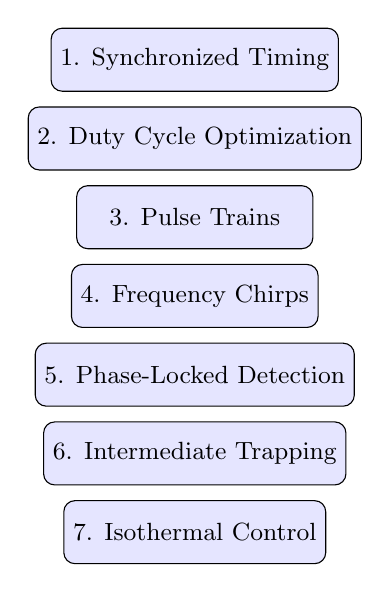
\begin{tikzpicture}[
    category/.style={rectangle, draw, rounded corners, minimum width=3cm, minimum height=0.8cm, text centered, font=\small, fill=blue!10}
]
    \node[category] (sync) at (0,5) {1. Synchronized Timing};
    \node[category] (duty) at (0,4) {2. Duty Cycle Optimization};
    \node[category] (train) at (0,3) {3. Pulse Trains};
    \node[category] (chirp) at (0,2) {4. Frequency Chirps};
    \node[category] (phase) at (0,1) {5. Phase-Locked Detection};
    \node[category] (trap) at (0,0) {6. Intermediate Trapping};
    \node[category] (iso) at (0,-1) {7. Isothermal Control};
\end{tikzpicture}
\caption{Seven categories of pulse protocols}
\label{fig:categories}
\end{figure}

\newpage

%% ============================================================================
%%                    BRIEF DESCRIPTION OF DRAWINGS
%% ============================================================================

\section{BRIEF DESCRIPTION OF DRAWINGS}

\subsection*{Figure 1: Seven Categories of Pulse Protocols}
A diagram showing the seven categories of pulse protocols covered by the present invention.

\subsection*{Figure 2: Synchronized Pulse Timing}
Timing diagrams showing pulse synchronization with T-jump, rapid mixing, and pH-jump folding initiation.

\subsection*{Figure 3: Duty Cycle Optimization}
Diagrams illustrating different duty cycles and their effects on thermal load and resonant modulation.

\subsection*{Figure 4: Pulse Train Protocol}
Timing diagram for pulse train kinetic measurements.

\subsection*{Figure 5: Frequency-Chirped Pulse}
Time-frequency diagram of a chirped pulse sweeping through the resonance.

\subsection*{Figure 6: Phase-Locked Detection Scheme}
Block diagram of the phase-locked detection system.

\subsection*{Figure 7: Intermediate Trapping Protocol}
Timing diagram showing pulse application for trapping folding intermediates.

\subsection*{Figure 8: Isothermal Pulsing Control Loop}
Control system diagram for maintaining constant temperature during pulsed irradiation.

\newpage

%% ============================================================================
%%                      DETAILED DESCRIPTION
%% ============================================================================

\section{DETAILED DESCRIPTION OF THE PREFERRED EMBODIMENTS}

\subsection{Protocol 1: Synchronized Pulse Timing}

\subsubsection{Principle}

Protein folding is a multi-stage process. By synchronizing microwave pulses with the folding initiation event, specific stages of folding can be selectively modulated.

\subsubsection{Synchronization with Temperature Jump (T-Jump)}

T-jump folding initiation uses a laser pulse to rapidly heat the sample, causing cold-denatured or temperature-sensitive proteins to begin folding.

\begin{figure}[h]
\centering
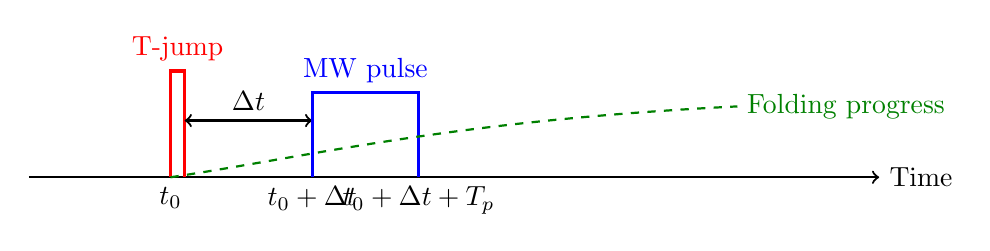
\begin{tikzpicture}[scale=0.9]
    % Time axis
    \draw[thick,->] (0,0) -- (12,0) node[right] {Time};
    
    % T-jump pulse
    \draw[very thick, red] (2,0) -- (2,1.5) -- (2.2,1.5) -- (2.2,0);
    \node[red, above] at (2.1,1.5) {T-jump};
    \node[below] at (2,0) {$t_0$};
    
    % Delay
    \draw[<->, thick] (2.2,0.8) -- (4,0.8);
    \node[above] at (3.1,0.8) {$\Delta t$};
    
    % MW pulse
    \draw[very thick, blue] (4,0) -- (4,1.2) -- (5.5,1.2) -- (5.5,0);
    \node[blue, above] at (4.75,1.2) {MW pulse};
    \node[below] at (4,0) {$t_0 + \Delta t$};
    \node[below] at (5.5,0) {$t_0 + \Delta t + T_p$};
    
    % Folding curve
    \draw[thick, green!50!black, dashed] (2,0) .. controls (4,0.3) and (6,0.8) .. (10,1);
    \node[green!50!black, right] at (10,1) {Folding progress};
    
\end{tikzpicture}
\caption{Synchronized pulse timing with T-jump initiation}
\label{fig:tjump_sync}
\end{figure}

\paragraph{Protocol Parameters:}
\begin{itemize}
\item T-jump pulse: 5--20 ns duration, $\Delta T = 5$--20$^\circ$C
\item Synchronization delay $\Delta t$: Programmable, 0 -- 100 ms
\item MW pulse frequency: 14.65 GHz (H$_2$O) or 10.4 GHz (D$_2$O)
\item MW pulse width $T_p$: 1 ns -- 10 ms
\item Trigger: Electrical sync from T-jump laser
\end{itemize}

\subsubsection{Synchronization with Rapid Mixing}

Rapid mixing uses stopped-flow or continuous-flow mixers to dilute a protein from denaturing conditions into folding-permissive buffer.

\paragraph{Protocol Parameters:}
\begin{itemize}
\item Mixing dead time: 100 $\mu$s -- 1 ms (instrument-dependent)
\item Synchronization delay $\Delta t$: Programmable, 0 -- 10 s
\item Trigger: Electrical sync from mixer stop/flow sensor
\end{itemize}

\subsubsection{Synchronization with pH Jump}

pH jump uses rapid addition of acid or base to change the protonation state of a protein, triggering folding.

\paragraph{Protocol Parameters:}
\begin{itemize}
\item pH change: Typically 2--3 units
\item Equilibration time: 10 $\mu$s -- 1 ms
\item Synchronization delay $\Delta t$: Programmable, 0 -- 10 s
\item Trigger: Electrical sync from injection valve
\end{itemize}

\subsubsection{Delay Scanning}

By varying the synchronization delay $\Delta t$ across multiple experiments, the effect of irradiation on different folding stages can be mapped:

\begin{equation}
M(\Delta t) = \text{Modulation as function of pulse delay}
\label{eq:delay_scan}
\end{equation}

This creates a ``folding modulation kinetic trace'' revealing which stages are most sensitive to resonant irradiation.

\subsection{Protocol 2: Duty Cycle Optimization}

\subsubsection{Definition}

The duty cycle $D$ is the fraction of time the microwave source is active:

\begin{equation}
D = \frac{T_{\text{on}}}{T_{\text{on}} + T_{\text{off}}} = \frac{T_{\text{on}}}{T_{\text{period}}}
\label{eq:duty_cycle}
\end{equation}

\subsubsection{Trade-offs}

\begin{table}[h]
\centering
\begin{tabular}{lcc}
\toprule
\textbf{Duty Cycle} & \textbf{Resonant Effect} & \textbf{Thermal Load} \\
\midrule
$D = 100\%$ (CW) & Maximum & Maximum \\
$D = 50\%$ & Moderate & 50\% of CW \\
$D = 10\%$ & Reduced & 10\% of CW \\
$D = 1\%$ & Minimal & 1\% of CW \\
\bottomrule
\end{tabular}
\caption{Duty cycle trade-offs}
\end{table}

\subsubsection{Optimal Duty Cycle Determination}

The optimal duty cycle balances resonant modulation against thermal effects:

\begin{equation}
D_{\text{opt}} = \arg\max_D \left[ \frac{M(D)}{\Delta T(D)} \right]
\label{eq:optimal_duty}
\end{equation}

where $M(D)$ is the modulation magnitude and $\Delta T(D)$ is the temperature rise.

\begin{figure}[h]
\centering
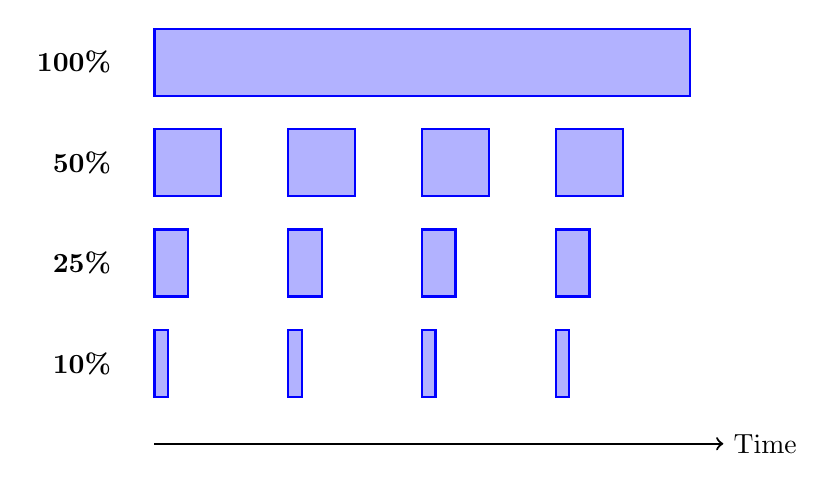
\begin{tikzpicture}[scale=0.85]
    % 100% duty cycle
    \node[left] at (-0.5,4.5) {\textbf{100\%}};
    \draw[thick, blue, fill=blue!30] (0,4) rectangle (8,5);
    
    % 50% duty cycle
    \node[left] at (-0.5,3) {\textbf{50\%}};
    \foreach \x in {0,2,4,6} {
        \draw[thick, blue, fill=blue!30] (\x,2.5) rectangle (\x+1,3.5);
    }
    
    % 25% duty cycle
    \node[left] at (-0.5,1.5) {\textbf{25\%}};
    \foreach \x in {0,2,4,6} {
        \draw[thick, blue, fill=blue!30] (\x,1) rectangle (\x+0.5,2);
    }
    
    % 10% duty cycle
    \node[left] at (-0.5,0) {\textbf{10\%}};
    \foreach \x in {0,2,4,6} {
        \draw[thick, blue, fill=blue!30] (\x,-0.5) rectangle (\x+0.2,0.5);
    }
    
    % Time axis
    \draw[thick,->] (0,-1.2) -- (8.5,-1.2) node[right] {Time};
    
\end{tikzpicture}
\caption{Different duty cycles: 100\%, 50\%, 25\%, and 10\%}
\label{fig:duty_cycles}
\end{figure}

\subsubsection{Adaptive Duty Cycle Control}

The duty cycle can be dynamically adjusted based on temperature feedback:

\begin{equation}
D(t) = D_{\text{max}} \times \left[ 1 - \frac{T(t) - T_{\text{set}}}{\Delta T_{\text{max}}} \right]
\label{eq:adaptive_duty}
\end{equation}

where $\Delta T_{\text{max}}$ is the maximum allowed temperature rise.

\subsection{Protocol 3: Pulse Train Methods}

\subsubsection{Single-Frequency Pulse Train}

A train of $N$ identical pulses at fixed spacing:

\begin{equation}
P(t) = P_0 \sum_{n=0}^{N-1} \Pi\left(\frac{t - nT_{\text{rep}}}{T_{\text{pulse}}}\right)
\label{eq:pulse_train}
\end{equation}

where $\Pi$ is the rectangular function, $T_{\text{rep}}$ is the repetition period, and $T_{\text{pulse}}$ is the pulse width.

\begin{figure}[h]
\centering
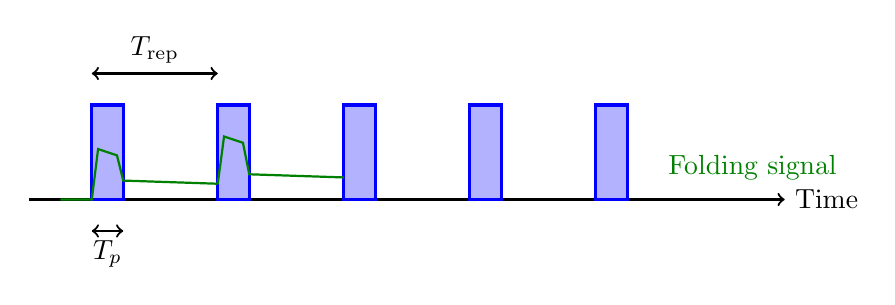
\begin{tikzpicture}[scale=0.8]
    % Time axis
    \draw[thick,->] (0,0) -- (12,0) node[right] {Time};
    
    % Pulses
    \foreach \x in {1,3,5,7,9} {
        \draw[very thick, blue, fill=blue!30] (\x,0) rectangle (\x+0.5,1.5);
    }
    
    % Labels
    \draw[<->, thick] (1,2) -- (3,2);
    \node[above] at (2,2) {$T_{\text{rep}}$};
    
    \draw[<->, thick] (1,-0.5) -- (1.5,-0.5);
    \node[below] at (1.25,-0.5) {$T_p$};
    
    % Folding signal
    \draw[thick, green!50!black] (0.5,0) -- (1,0) -- (1.1,0.8) -- (1.4,0.7) -- (1.5,0.3) -- (3,0.25);
    \draw[thick, green!50!black] (3,0.25) -- (3.1,1) -- (3.4,0.9) -- (3.5,0.4) -- (5,0.35);
    
    \node[green!50!black, right] at (10,0.5) {Folding signal};
    
\end{tikzpicture}
\caption{Pulse train with folding signal response}
\label{fig:pulse_train}
\end{figure}

\subsubsection{Applications of Pulse Trains}

\begin{enumerate}[label=(\arabic*)]
\item \textbf{Kinetic rate determination:} Varying $T_{\text{rep}}$ reveals characteristic folding timescales.

\item \textbf{Signal averaging:} Multiple pulses improve signal-to-noise ratio.

\item \textbf{Dose-response characterization:} Varying $N$ determines cumulative effect.

\item \textbf{Recovery time measurement:} Time between pulses when effect ``wears off.''
\end{enumerate}

\subsubsection{Logarithmic Spacing}

For characterizing processes spanning many decades in time:

\begin{equation}
t_n = t_0 \times 10^{n/k}
\label{eq:log_spacing}
\end{equation}

where $k$ determines the number of points per decade.

\subsection{Protocol 4: Frequency-Chirped Pulses}

\subsubsection{Linear Chirp}

A frequency-chirped pulse sweeps through a range of frequencies during the pulse:

\begin{equation}
f(t) = f_0 + \frac{\Delta f}{T_{\text{pulse}}} \times t
\label{eq:linear_chirp}
\end{equation}

where $f_0$ is the starting frequency and $\Delta f$ is the total frequency sweep.

\begin{figure}[h]
\centering
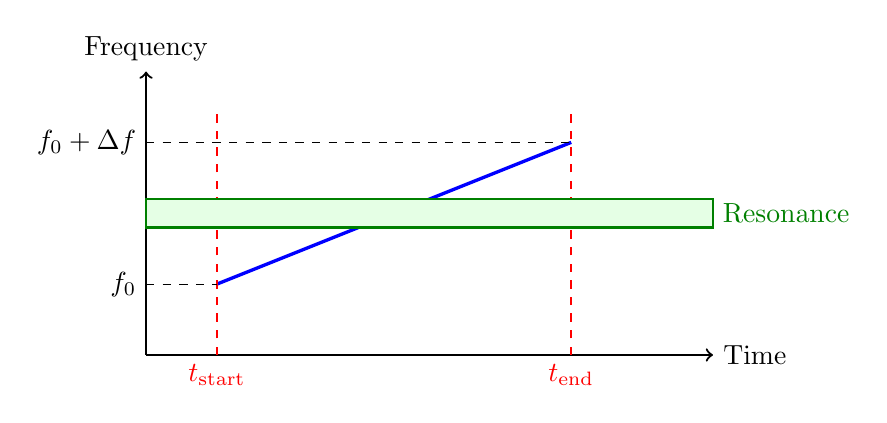
\begin{tikzpicture}[scale=0.9]
    % Axes
    \draw[thick,->] (0,0) -- (8,0) node[right] {Time};
    \draw[thick,->] (0,0) -- (0,4) node[above] {Frequency};
    
    % Chirp
    \draw[very thick, blue] (1,1) -- (6,3);
    
    % Pulse envelope
    \draw[thick, red, dashed] (1,0) -- (1,3.5);
    \draw[thick, red, dashed] (6,0) -- (6,3.5);
    \node[red, below] at (1,0) {$t_{\text{start}}$};
    \node[red, below] at (6,0) {$t_{\text{end}}$};
    
    % Frequency labels
    \node[left] at (0,1) {$f_0$};
    \node[left] at (0,3) {$f_0 + \Delta f$};
    \draw[dashed] (0,1) -- (1,1);
    \draw[dashed] (0,3) -- (6,3);
    
    % Resonance band
    \draw[thick, green!50!black, fill=green!10] (0,1.8) rectangle (8,2.2);
    \node[green!50!black, right] at (8,2) {Resonance};
    
\end{tikzpicture}
\caption{Linear frequency chirp sweeping through resonance}
\label{fig:chirp}
\end{figure}

\subsubsection{Applications of Chirped Pulses}

\begin{enumerate}[label=(\arabic*)]
\item \textbf{Broadband excitation:} Ensures resonance is hit even if exact frequency is uncertain.

\item \textbf{Adiabatic passage:} Slow chirp through resonance can achieve complete population inversion.

\item \textbf{Resonance mapping:} Time-resolved detection during chirp reveals resonance position.

\item \textbf{Isotope-blind operation:} Chirp covering both H$_2$O and D$_2$O frequencies works with mixed solvents.
\end{enumerate}

\subsubsection{Chirp Parameters}

\begin{table}[h]
\centering
\begin{tabular}{lll}
\toprule
\textbf{Parameter} & \textbf{Typical Value} & \textbf{Range} \\
\midrule
Start frequency $f_0$ & 12 GHz & 8--14 GHz \\
Frequency sweep $\Delta f$ & 5 GHz & 2--10 GHz \\
Chirp duration & 1--100 $\mu$s & 100 ns -- 1 ms \\
Chirp rate & 0.05--5 GHz/$\mu$s & --- \\
\bottomrule
\end{tabular}
\caption{Typical chirp parameters}
\end{table}

\subsection{Protocol 5: Phase-Locked Detection}

\subsubsection{Principle}

Phase-locked detection (also called lock-in detection) improves signal-to-noise ratio by modulating the microwave source and detecting only the component of the folding signal at the modulation frequency.

\subsubsection{Implementation}

\begin{figure}[h]
\centering
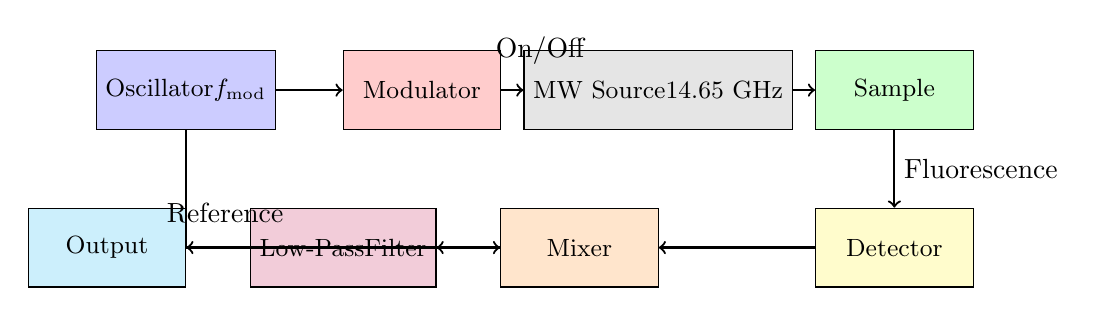
\begin{tikzpicture}[
    block/.style={rectangle, draw, minimum width=2cm, minimum height=1cm, text centered, font=\small},
    arrow/.style={->, thick}
]
    % Blocks
    \node[block, fill=blue!20] (osc) at (0,2) {Oscillator\\$f_{\text{mod}}$};
    \node[block, fill=red!20] (mod) at (3,2) {Modulator};
    \node[block, fill=gray!20] (mw) at (6,2) {MW Source\\14.65 GHz};
    \node[block, fill=green!20] (sample) at (9,2) {Sample};
    \node[block, fill=yellow!20] (det) at (9,0) {Detector};
    \node[block, fill=orange!20] (mixer) at (5,0) {Mixer};
    \node[block, fill=purple!20] (lpf) at (2,0) {Low-Pass\\Filter};
    \node[block, fill=cyan!20] (output) at (-1,0) {Output};
    
    % Arrows
    \draw[arrow] (osc) -- (mod);
    \draw[arrow] (mod) -- (mw);
    \draw[arrow] (mw) -- (sample);
    \draw[arrow] (sample) -- (det);
    \draw[arrow] (det) -- (mixer);
    \draw[arrow] (osc) -- (0,0) -- (mixer);
    \draw[arrow] (mixer) -- (lpf);
    \draw[arrow] (lpf) -- (output);
    
    % Labels
    \node[above] at (4.5,2.2) {On/Off};
    \node[right] at (9,1) {Fluorescence};
    \node[above] at (0.5,0.2) {Reference};
    
\end{tikzpicture}
\caption{Phase-locked detection scheme}
\label{fig:lockin}
\end{figure}

\paragraph{Protocol Parameters:}
\begin{itemize}
\item Modulation frequency $f_{\text{mod}}$: 100 Hz -- 100 kHz
\item Lock-in time constant: $\tau = 1/(2\pi f_{\text{mod}})$ to $10/f_{\text{mod}}$
\item Phase: 0$^\circ$ (in-phase) and 90$^\circ$ (quadrature) detection
\end{itemize}

\subsubsection{Advantages}

\begin{enumerate}[label=(\arabic*)]
\item \textbf{Noise rejection:} Rejects noise at frequencies other than $f_{\text{mod}}$.
\item \textbf{Baseline elimination:} Removes static background signals.
\item \textbf{Small signal detection:} Can detect modulation amplitudes $<$1\% of baseline.
\item \textbf{Thermal discrimination:} Slow thermal effects are filtered out.
\end{enumerate}

\subsection{Protocol 6: Intermediate Trapping}

\subsubsection{Principle}

By applying a microwave pulse at a precisely timed moment during folding, the protein can be ``frozen'' in an intermediate state. The resonant coupling disrupts the molecular gate, preventing further conformational transitions.

\subsubsection{Trapping Protocol}

\begin{figure}[h]
\centering
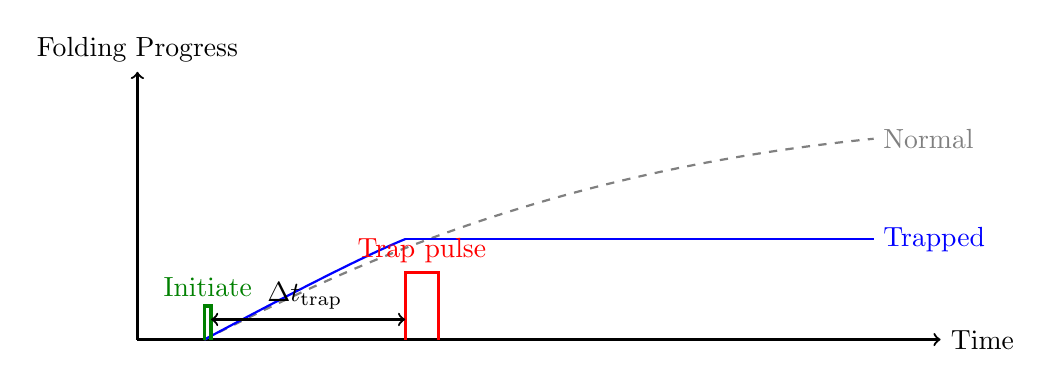
\begin{tikzpicture}[scale=0.85]
    % Time axis
    \draw[thick,->] (0,0) -- (12,0) node[right] {Time};
    \draw[thick,->] (0,0) -- (0,4) node[above] {Folding Progress};
    
    % Normal folding curve
    \draw[thick, gray, dashed] (1,0) .. controls (3,1) and (6,2.5) .. (11,3);
    \node[gray, right] at (11,3) {Normal};
    
    % Trapped folding
    \draw[thick, blue] (1,0) .. controls (2.5,0.8) and (3.5,1.3) .. (4,1.5);
    \draw[thick, blue] (4,1.5) -- (11,1.5);
    \node[blue, right] at (11,1.5) {Trapped};
    
    % Trap pulse
    \draw[very thick, red] (4,0) -- (4,1) -- (4.5,1) -- (4.5,0);
    \node[red, above] at (4.25,1) {Trap pulse};
    
    % Initiation
    \draw[very thick, green!50!black] (1,0) -- (1,0.5) -- (1.1,0.5) -- (1.1,0);
    \node[green!50!black, above] at (1.05,0.5) {Initiate};
    
    % Delay
    \draw[<->, thick] (1.1,0.3) -- (4,0.3);
    \node[above] at (2.5,0.3) {$\Delta t_{\text{trap}}$};
    
\end{tikzpicture}
\caption{Intermediate trapping protocol}
\label{fig:trapping}
\end{figure}

\paragraph{Protocol Steps:}
\begin{enumerate}[label=(\arabic*)]
\item Initiate folding (T-jump, mixing, pH-jump, etc.).
\item Wait for delay time $\Delta t_{\text{trap}}$ corresponding to desired intermediate.
\item Apply trapping pulse at jamming frequency.
\item Maintain continuous irradiation to prevent escape from trapped state.
\item Characterize intermediate using spectroscopic methods.
\item Optionally, turn off irradiation to allow completion of folding.
\end{enumerate}

\subsubsection{Trap Pulse Parameters}

\begin{table}[h]
\centering
\begin{tabular}{lll}
\toprule
\textbf{Parameter} & \textbf{Typical Value} & \textbf{Notes} \\
\midrule
Trap pulse onset $\Delta t_{\text{trap}}$ & 1 $\mu$s -- 100 ms & Stage-dependent \\
Trap pulse width & 10 ns -- 10 ms & Must exceed $\tau_{19}$ \\
Trap pulse power & 1--10 W & Sample-dependent \\
Maintenance power & 0.1--1 W & Lower than trap \\
Frequency & 14.65 GHz (H$_2$O) & Or 10.4 GHz (D$_2$O) \\
\bottomrule
\end{tabular}
\caption{Intermediate trapping pulse parameters}
\end{table}

\subsubsection{Applications}

\begin{enumerate}[label=(\arabic*)]
\item \textbf{Structural biology:} Trap and characterize normally transient intermediates.
\item \textbf{Drug discovery:} Identify druggable intermediate states.
\item \textbf{Misfolding studies:} Trap misfolding intermediates for aggregation studies.
\item \textbf{Mechanism elucidation:} Map folding pathway by trapping at different times.
\end{enumerate}

\subsection{Protocol 7: Isothermal Pulsing Control}

\subsubsection{Challenge}

Pulsed irradiation deposits energy in the sample, causing temperature fluctuations. For rigorous comparison of resonant vs.\ thermal effects, the sample temperature must remain constant.

\subsubsection{Control Algorithm}

\begin{enumerate}[label=(\arabic*)]
\item \textbf{Predictive cooling:} Before each pulse, apply pre-cooling to bring sample below $T_{\text{set}}$.

\item \textbf{Real-time feedback:} During pulse, monitor temperature and adjust pulse width/power.

\item \textbf{Inter-pulse equilibration:} Ensure temperature returns to baseline between pulses.
\end{enumerate}

\begin{figure}[h]
\centering
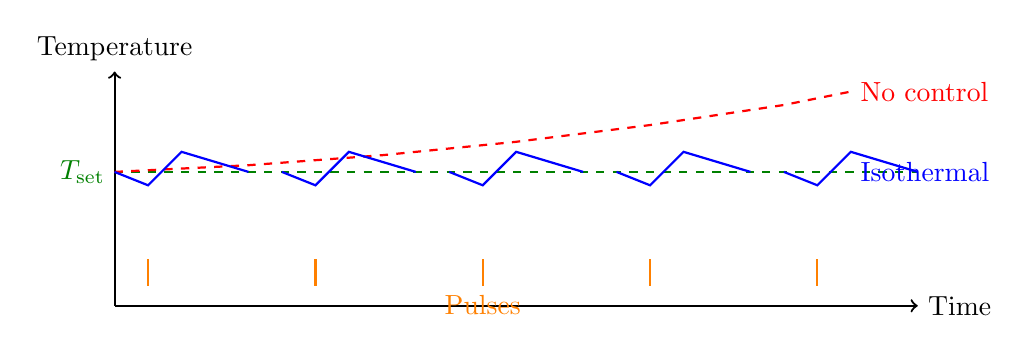
\begin{tikzpicture}[scale=0.85]
    % Time axis
    \draw[thick,->] (0,0) -- (12,0) node[right] {Time};
    \draw[thick,->] (0,0) -- (0,3.5) node[above] {Temperature};
    
    % Setpoint
    \draw[thick, green!50!black, dashed] (0,2) -- (12,2);
    \node[green!50!black, left] at (0,2) {$T_{\text{set}}$};
    
    % Without control (rising)
    \draw[thick, red, dashed] (0,2) -- (2,2.1) -- (4,2.25) -- (6,2.45) -- (8,2.7) -- (10,3) -- (11,3.2);
    \node[red, right] at (11,3.2) {No control};
    
    % With isothermal control
    \draw[thick, blue] (0,2);
    \foreach \x in {0,2.5,5,7.5,10} {
        \draw[thick, blue] (\x,2) -- (\x+0.5,1.8) -- (\x+1,2.3) -- (\x+2,2);
    }
    \node[blue, right] at (11,2) {Isothermal};
    
    % Pulses
    \foreach \x in {0.5,3,5.5,8,10.5} {
        \draw[thick, orange] (\x,0.3) -- (\x,0.7);
    }
    \node[orange, below] at (5.5,0.3) {Pulses};
    
\end{tikzpicture}
\caption{Isothermal pulsing control: Temperature maintained despite pulsed irradiation}
\label{fig:isothermal}
\end{figure}

\subsubsection{Control Equations}

Pre-cooling setpoint:
\begin{equation}
T_{\text{pre}} = T_{\text{set}} - \alpha \times P_{\text{pulse}} \times T_{\text{pulse}}
\label{eq:precool}
\end{equation}

where $\alpha$ is a calibrated heating coefficient (K/J).

Inter-pulse cooling time:
\begin{equation}
t_{\text{cool}} \geq \frac{C_{\text{sample}}}{k_{\text{cool}}} \times \ln\left(\frac{T_{\text{peak}} - T_{\text{set}}}{0.01^\circ\text{C}}\right)
\label{eq:cool_time}
\end{equation}

where $C_{\text{sample}}$ is the sample heat capacity and $k_{\text{cool}}$ is the cooling rate constant.

\subsubsection{Isothermal Compliance Criteria}

For a protocol to be considered ``isothermal'':

\begin{enumerate}[label=(\arabic*)]
\item Peak temperature excursion: $|T_{\text{peak}} - T_{\text{set}}| < 0.5^\circ$C
\item Time-averaged temperature: $|\langle T \rangle - T_{\text{set}}| < 0.1^\circ$C
\item RMS temperature fluctuation: $\sqrt{\langle (T - T_{\text{set}})^2 \rangle} < 0.2^\circ$C
\end{enumerate}

\subsection{Combined Protocols}

The seven protocols can be combined for advanced applications:

\subsubsection{Example: Phase-Locked Intermediate Trapping}

\begin{enumerate}[label=(\arabic*)]
\item Initiate folding with T-jump.
\item Wait for delay $\Delta t_{\text{trap}}$.
\item Apply modulated trap pulse train (Protocol 5 + 6).
\item Use lock-in detection to confirm trapping.
\item Characterize intermediate.
\end{enumerate}

\subsubsection{Example: Isothermal Chirped Pulse Scan}

\begin{enumerate}[label=(\arabic*)]
\item Apply frequency-chirped pulses (Protocol 4).
\item Use isothermal control (Protocol 7) to prevent heating.
\item Record resonance frequency from time-resolved detection.
\item Repeat with D$_2$O to confirm $\sqrt{2}$ shift.
\end{enumerate}

\newpage

%% ============================================================================
%%                              CLAIMS
%% ============================================================================

\section{CLAIMS}

What is claimed is:

\subsection{Synchronized Timing Claims}

\begin{enumerate}[label=\textbf{\arabic*.}]

\item A method for modulating protein folding using synchronized pulsed irradiation, comprising:
\begin{enumerate}[label=(\alph*)]
\item initiating protein folding by an initiation event selected from temperature jump, rapid mixing, pH jump, photolysis, and pressure jump;
\item detecting the initiation event and generating a trigger signal;
\item after a programmable delay $\Delta t$ following the trigger signal, applying a pulse of electromagnetic radiation at a frequency in the range of 12 to 17 GHz; and
\item measuring the effect of the pulse on protein folding.
\end{enumerate}

\item The method of claim 1, wherein the frequency is approximately 14.65 GHz for H$_2$O samples or 10.4 GHz for D$_2$O samples.

\item The method of claim 1, wherein the programmable delay $\Delta t$ is in the range of 0 to 10 seconds.

\item The method of claim 1, further comprising varying the delay $\Delta t$ across multiple experiments to map folding stage sensitivity to irradiation.

\item The method of claim 1, wherein the initiation event is a temperature jump induced by a laser pulse.

\end{enumerate}

\subsection{Duty Cycle Claims}

\begin{enumerate}[label=\textbf{\arabic*.}]
\setcounter{enumi}{5}

\item A method for optimizing pulsed irradiation for protein folding modulation, comprising:
\begin{enumerate}[label=(\alph*)]
\item applying pulsed irradiation at a duty cycle $D$ defined as the ratio of on-time to total period;
\item measuring folding modulation magnitude $M(D)$ as a function of duty cycle;
\item measuring temperature rise $\Delta T(D)$ as a function of duty cycle; and
\item selecting an optimal duty cycle $D_{\text{opt}}$ that maximizes the ratio $M(D)/\Delta T(D)$.
\end{enumerate}

\item The method of claim 6, wherein the duty cycle is in the range of 1\% to 100\%.

\item The method of claim 6, further comprising dynamically adjusting the duty cycle based on real-time temperature feedback to maintain isothermal conditions.

\end{enumerate}

\subsection{Pulse Train Claims}

\begin{enumerate}[label=\textbf{\arabic*.}]
\setcounter{enumi}{8}

\item A method for characterizing protein folding kinetics using pulse trains, comprising:
\begin{enumerate}[label=(\alph*)]
\item applying a train of $N$ pulses at the jamming frequency with pulse width $T_{\text{pulse}}$ and repetition period $T_{\text{rep}}$;
\item measuring the folding response after each pulse; and
\item analyzing the response pattern to determine folding kinetic parameters.
\end{enumerate}

\item The method of claim 9, wherein the repetition period $T_{\text{rep}}$ is varied logarithmically to span multiple decades of time.

\item The method of claim 9, wherein $N$ is in the range of 2 to 1000 pulses.

\end{enumerate}

\subsection{Chirped Pulse Claims}

\begin{enumerate}[label=\textbf{\arabic*.}]
\setcounter{enumi}{11}

\item A method for broadband resonant excitation of protein folding modulation, comprising:
\begin{enumerate}[label=(\alph*)]
\item generating a frequency-chirped pulse that sweeps from a starting frequency $f_0$ to an ending frequency $f_0 + \Delta f$ over a pulse duration $T_{\text{chirp}}$;
\item applying the chirped pulse to a protein sample; and
\item detecting the folding response during or after the pulse.
\end{enumerate}

\item The method of claim 12, wherein $f_0$ is in the range of 8 to 14 GHz and $\Delta f$ is in the range of 2 to 10 GHz.

\item The method of claim 12, wherein the chirp covers both the H$_2$O jamming frequency ($\sim$14.65 GHz) and the D$_2$O jamming frequency ($\sim$10.4 GHz).

\item The method of claim 12, further comprising time-resolved detection during the chirp to identify the resonant frequency.

\end{enumerate}

\subsection{Phase-Locked Detection Claims}

\begin{enumerate}[label=\textbf{\arabic*.}]
\setcounter{enumi}{15}

\item A method for enhanced detection of protein folding modulation, comprising:
\begin{enumerate}[label=(\alph*)]
\item modulating the microwave irradiation at a modulation frequency $f_{\text{mod}}$;
\item detecting the folding signal (e.g., fluorescence);
\item mixing the detected signal with a reference signal at $f_{\text{mod}}$;
\item applying a low-pass filter to extract the component at $f_{\text{mod}}$; and
\item outputting the filtered signal as the modulation amplitude.
\end{enumerate}

\item The method of claim 16, wherein the modulation frequency $f_{\text{mod}}$ is in the range of 100 Hz to 100 kHz.

\item The method of claim 16, further comprising detecting both in-phase and quadrature components.

\end{enumerate}

\subsection{Intermediate Trapping Claims}

\begin{enumerate}[label=\textbf{\arabic*.}]
\setcounter{enumi}{18}

\item A method for trapping protein folding intermediates, comprising:
\begin{enumerate}[label=(\alph*)]
\item initiating protein folding;
\item waiting for a predetermined trap delay $\Delta t_{\text{trap}}$ corresponding to a desired intermediate state;
\item applying a trap pulse of electromagnetic radiation at the jamming frequency;
\item maintaining irradiation to prevent escape from the intermediate state; and
\item characterizing the trapped intermediate.
\end{enumerate}

\item The method of claim 19, wherein the trap delay $\Delta t_{\text{trap}}$ is in the range of 1 microsecond to 100 milliseconds.

\item The method of claim 19, wherein the trap pulse width is in the range of 10 nanoseconds to 10 milliseconds.

\item The method of claim 19, wherein the intermediate is characterized by one or more of: fluorescence spectroscopy, circular dichroism, NMR, mass spectrometry, and cryo-electron microscopy.

\item The method of claim 19, further comprising releasing the intermediate by turning off irradiation and observing completion of folding.

\end{enumerate}

\subsection{Isothermal Pulsing Claims}

\begin{enumerate}[label=\textbf{\arabic*.}]
\setcounter{enumi}{23}

\item A method for maintaining isothermal conditions during pulsed irradiation of protein samples, comprising:
\begin{enumerate}[label=(\alph*)]
\item applying predictive pre-cooling before each pulse to offset anticipated heating;
\item monitoring sample temperature during and after each pulse;
\item adjusting cooling power to return sample to setpoint temperature between pulses; and
\item verifying that peak temperature excursion is less than a predetermined threshold.
\end{enumerate}

\item The method of claim 24, wherein the peak temperature excursion threshold is 0.5$^\circ$C.

\item The method of claim 24, wherein the time-averaged temperature is maintained within 0.1$^\circ$C of the setpoint.

\item The method of claim 24, further comprising adjusting pulse power or duty cycle if temperature control is insufficient.

\end{enumerate}

\subsection{Combination Claims}

\begin{enumerate}[label=\textbf{\arabic*.}]
\setcounter{enumi}{27}

\item A method combining synchronized timing and intermediate trapping, comprising the method of claim 1 wherein the pulse is a trap pulse according to claim 19.

\item A method combining phase-locked detection and intermediate trapping, comprising the method of claim 16 wherein the modulated irradiation is applied as a trap according to claim 19.

\item A method combining chirped pulses and isothermal control, comprising the method of claim 12 wherein isothermal conditions are maintained according to claim 24.

\end{enumerate}

\newpage

%% ============================================================================
%%                         ABSTRACT
%% ============================================================================

\section*{ABSTRACT}
\addcontentsline{toc}{section}{ABSTRACT}

Methods for applying pulsed electromagnetic radiation at a resonant jamming frequency (approximately 14.65 GHz for H$_2$O, 10.4 GHz for D$_2$O) to modulate protein folding dynamics. The methods comprise seven protocol categories: (1) synchronized pulse timing relative to folding initiation events (temperature jump, rapid mixing, pH jump) with programmable delays enabling stage-selective modulation; (2) duty cycle optimization balancing folding modulation against thermal load with adaptive control; (3) pulse train protocols with variable repetition periods for kinetic characterization; (4) frequency-chirped pulses for broadband resonance excitation and resonance mapping; (5) phase-locked detection schemes for enhanced signal-to-noise ratio and thermal discrimination; (6) intermediate trapping protocols using precisely timed pulses to arrest folding at specific stages for characterization; and (7) isothermal pulsing control rules using predictive pre-cooling and real-time feedback to maintain constant sample temperature despite pulsed irradiation. The protocols may be combined for advanced applications. Pulse timing parameters are derived from the molecular gate timescale ($\tau_{19} \approx 68$ ps). Applications include structural biology research, drug discovery, biopharmaceutical manufacturing, and therapeutic intervention in protein misfolding diseases.

\vspace{1in}

\begin{center}
\textbf{--- END OF SPECIFICATION ---}
\end{center}

\newpage

%% ============================================================================
%%                         INVENTOR DECLARATION
%% ============================================================================

\section*{INVENTOR DECLARATION}
\addcontentsline{toc}{section}{INVENTOR DECLARATION}

I, Jonathan Washburn, declare that:

\begin{enumerate}[label=(\arabic*)]
\item I am the original and sole inventor of the pulse protocol methods described and claimed in this application.

\item I have reviewed the above specification and claims and believe them to be accurate and complete.

\item I believe the claimed invention to be novel, useful, and non-obvious over the prior art.

\item I authorize the filing of this provisional patent application to establish a priority date.
\end{enumerate}

\vspace{1in}

\noindent\textbf{Inventor Signature:} \hrulefill

\vspace{0.5in}

\noindent\textbf{Name:} Jonathan Washburn

\noindent\textbf{Email:} washburn.jonathan@gmail.com

\noindent\textbf{Date:} \hrulefill

\vspace{1in}

\begin{center}
\textit{This document is intended for provisional patent application filing purposes.\\
All information contained herein is confidential and proprietary.}
\end{center}

\end{document}
